\textbf{Texto de apoio para as questões 21 e 22}\par\medskip
\textbf{A simple guide to getting a good night’s sleep}\par
\textit{If you struggle to drop off, or wake up for hours in the night, these straightforward steps from a sleep expert should solve the problem}\par
Alanna Hare — Sunday 15th of September, 2019\par\medskip
\begin{figure}[htbp]
\centering
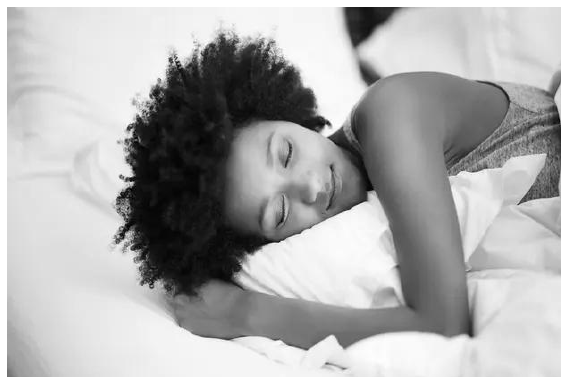
\includegraphics[width=0.56\linewidth]{static/simulados/coluni/figuras/2020/questao-21/figura-1.png}
\end{figure}
Photograph: PeopleImages/Getty Images.\par\medskip

People who sleep well do not actively try to get to sleep; they get into bed and sleep arrives. So, the main thing is not to try to go to sleep. If you are actively trying, sleep will get further out of reach. Have a regular bedtime and getting-up time, as it trains your body into a rhythm.\par
Get ready for sleep 30 minutes or so before bed with a wind-down routine. This can be whatever works for you – for example, taking off your makeup, getting changed and reading. The aim is to find something that helps you switch off from the day. Turn off devices 30 to 60 minutes before bed, partly because there is evidence to suggest the blue light they emit can switch off the natural sleep hormone melatonin, but also to take your mind off social media, the news or work. If you use your phone as an alarm, it may not be practical to keep it out of the bedroom, but avoid using it once you are settling down to sleep.\par
If you wake in the night, trust that your natural sleep drive will get you back to sleep at some point. Avoid clock-watching, which can exacerbate anxiety. If you start to feel anxious, get up and do something relaxing elsewhere – read a book or do a mindfulness activity – and then return to bed once you feel sleepy again.\par
If you are still struggling with your sleep and it is starting to affect your daily life, see your doctor or a sleep specialist who can work with you to provide effective treatments.\par
Alanna Hare, a consultant in sleep disorders at Royal Brompton hospital, London.\par
Disponível em: \url{https://www.theguardian.com/lifeandstyle/2019/sep/15/a-simple-guide-to-getting-a-good-nights-sleep}. Acesso em: 16 set. 2019. (Adaptado)\par\medskip

\textbf{COLUNI 2020 -- Questão 22}\par\medskip Com base no texto lido, observe as seguintes afirmativas:\begin{enumerate}
\item[I.] Adote uma rotina relaxante cerca de trinta minutos antes de ir para a cama.
\item[II.] Desligue todos os equipamentos eletrônicos cerca de uma hora antes de ir dormir.
\item[III.] Tenha um relógio sempre à vista no seu quarto para evitar ansiedade.
\item[IV.] Caso se sinta ansioso durante a noite, leia um livro.
\item[V.] Se a dificuldade para dormir persistir, procure um médico.
\end{enumerate}
Está CORRETO o que se afirma apenas em:\begin{enumerate}
\item I, II, III e IV.
\item I, III e V.
\item I, II, IV e V.
\item II, III, IV e V.\end{enumerate}